\documentclass[bsc,singlespacing,parskip,deptreport,twoside,frontabs]{infthesis}

\usepackage{natbib}
\usepackage{graphicx}
\usepackage{listings}
\usepackage{amsmath}
\usepackage{xcolor}
\lstset{language=Python, breaklines=true, postbreak=\raisebox{0ex}[0ex][0ex]{\ensuremath{\color{red}\hookrightarrow\space}}}
\begin{document}



\title{Automatic Harmonic Analysis of Jazz Melodies}

\author{Finlay McAfee - s1220880}

\course{Master of Informatics}
\project{{\bf MInf Project (Part 1)}}

\date{\today
}

\abstract{
This report presents a system for the automatic harmonic analysis of jazz melodies. It is a baseline Hidden Markov Model approach, upon which a more sophisticated, grammar based approach will be implemented in the next year of this project. Multiple local 'emission' models are proposed and implemented, with the most effective being based on decision trees and chord tones, see Section 3.3.2.2 for a detailed description of this specific model.  
}

\maketitle

\begin{acknowledgements}
I would like to thank Mark Steedman and Andrew McLeod for their advice and guidance on this project.
\end{acknowledgements}

\tableofcontents

\pagenumbering{arabic}

\chapter{Introduction}

The aim of this project is to build a system that will analyse a jazz melody and determine the underlying chord sequence. The purpose of this report is to give a summary of the work that has been completed this year and to outline the future work that shall be done in the following year of this project.

The proposed system to tackle this task is based on the assumption that harmonic analysis of musical input is analogous to automatic speech recognition in the field of natural language processing. This allows the task to be divided into two distinct modules, a transition (language) model and an emission (acoustic) model. The transition model is the probability of transitioning from one chord to another. The emission model is the probability of the current chord generating the observed notes. This kind of structure allows for a probabilistic generative model, where given a chord sequence we can model the generation of the more complex note sequence.

\begin{equation}
\label{eq}
P(o_t) = P(o_t | s_t)P(s_t | s_{1:t}) 
\end{equation}

The task of the first year of this project is to design a baseline Hidden Markov Model system, where the transition model is the first order markov assumption:

\begin{equation}
\label{hmm_eq}
P(s_t | s_{1:t}) = P(s_t | s_{t-1}) 
\end{equation}

This allows the focus to be on designing an emission model that best captures the relationship between the observations and the underlying chord. This process can be split into two tasks, feature extraction and segment classification. The approach taken to both will be detailed as well as planned future improvements.

The end goal of this project is to incorporate the best determined emission model into a grammar based harmonic analysis of jazz, using the Combinatory Categorical Grammars (CCGs) presented by \cite{ccg}. This will be achieved in the following year.

A brief overview of the relevant literature is given in Chapter 2, followed by a comprehensive System Description in Chapter 3. Chapter 4 goes into detail in terms of implementation and Chapter 5 presents the results of tests carried out over the various models. Finally Chapter 6 details the plan for the next year of this project.

\chapter{Literature Review}

A brief review of previous work on chord progression estimation and related works will be presented in this chapter.

The field of automatic harmonic analysis of music has seen a wide range of research in the past few decades. Much of this stems from the interpretation of music as a form of language, or at least recognising the similarities between music and natural language and exploiting them to achieve certain tasks. The works of \cite{winograd1968linguistics} and \cite{forte1967syntax} were some of the first applications of computational linguistic theory to the field of music, inspired by the pioneering work of Noam Chomsky on the formal definitions of languages and syntax \cite[]{lees1957syntactic}. In \cite{winograd1968linguistics} a generative grammar for the parsing of a harmonic phrase was proposed, using an adaptation of the formalism of tonal harmony proposed by \cite{forte1962tonal}. This mechanism was capable of automatically parsing chorales.

An alternative method of harmonic analysis, introduced by \cite{schenker1979harmony}, was used in another computationally assisted, automatic parsing of music in \cite{smoliar1979computer}. Similar to the above, Smolier applied existing NLP parsing techniques to a grammatical formalism of tonal music.

Logic based approaches have also been attempted. In \cite{ebciouglu1990expert} an expert system for the harmonic analysis of chorales is proposed, based on first order predicate logic. This was expanded on by \cite{maxwell1992expert}, where a full approach applicable to all tonal music was presented. A similar hierarchical logical representation for the computational analysis of music was proposed by \cite{smaill1993hierarchical}.

The development of probabilistic machine learning algorithms allowed for a more statistical approach to harmonic analysis to be developed. The work of \cite{laden1989representation} applies neural networks to chord classification, focusing on the problem of how to best represent pitch. A more qualitative perception model for musical learning is presented in \cite{widmer1992qualitative}.

A popular and successful method of probabilistic harmonic analysis is the HMM based approach. The harmonic analysis of chorales proposed in \cite{allan2005harmonising} uses HMM probabilistic inference. In \cite{lee2004ring} an HMM based method for chord generation from a hummed input is presented. A simple frequency count based HMM is used in the chordal analysis of the MySong application by Microsoft \cite[]{mysong}, a system that automatically generates an accompaniment for a real-time vocal input. A more complex HMM based system is utilised by \cite{ryynanen2008automatic} in the automatic transcription of melody and chords from the first eight Beatles albums.

The HMM based approach shall form the basis of the baseline model for this project, where in the following year the markov assumption shall be replaced with a more complex grammar based language model. 

In more recent years, a template based approach to chordal analysis has been proposed, notably in the work of \cite{pardo2002algorithms}, \cite{oudre2009template} and \cite{oudre2011probabilistic}. This method moves away from more statistical techniques and instead assigns a rule-based scoring to a frame, based on whether the observed notes are present in the stored chord model template.

More complex hybrid approaches have also been attempted. A combination of neo-Riemannian transformations, Markov chains and Support Vector Machines are used in \cite{chuan2007hybrid} for the generation of style-specific accompaniment. This method uses machine learning techniques to decide how probable it is that an observed note is a 'chord tone' for the current chord and is the inspiration for one of the proposed emission models in this report.  

A method that uses additional structural information for chordal analysis is proposed in \cite{struct}. The success of this model supports the proposition that the additional structural CCG grammar, that will be implemented in the continuation of this project next year, will improve results.

It should be noted that the majority of these approaches assume pre-segmentation of the input into distinct chord segments for classification, as does the work presented in this report. A complete model of chordal analysis must take this aspect into account as well. There are many well researched methods for accomplishing this, a good review of a few of these is provided in \cite{pardo2002algorithms}.

\chapter{System Description}

This section outlines the structure of the proposed system. Each component will be summarised, along with its function in the complete system. For most components there are multiple possible models that were attempted, the following chapter will then present and analyse experiments done over these variations.

\section{General Overview}

As discussed in the introduction, the problem of assigning a sequence of chords to a sequence of notes is being treated in a similar way to speech recognition or Part-Of-Speech (POS) tagging in NLP \cite[]{cutting1992practical}. The probability of observing a note at time $t$ is assumed to be dependent on the probability of observing that note given the current underlying chord, see Figure 3.1, and the probability of that chord being generated by the preceding sequence of chords from time 0 to $t-1$, see Figure 3.2. These are referred to in this report as the emission model and the transition model respectively, see Equation \ref{eq}.

The problem is simplified in this project by assuming the data is already segmented into distinct chordal sections. That is, the input data sequence is segmented into lots of smaller sequences, each associated with a single chord in the progression. As mentioned in Chapter 2, see \cite{pardo2002algorithms} for an overview of the available segmentation algorithms for this process. Note a more comprehensive system would combine the segmentation and classification stages, this is a possible improvement that could be made next year.

The melody is hence modelled as a transition from one chord to another, where each chord is 'emitted' as a short sequence of notes. The emission model problem is treated in this project as a sequential machine learning task, where a single class (chord) is assigned to the entire sequence (segment). Hence attempts are made not to lose this sequential data. Section 3.3 will go over this in more detail. The transition model used in this first half of the project is based on a first order markov assumption, hence the entire model can be seen as an HMM. Section 3.4 will elaborate on this. The primary aim of next year's project is to do away with this simplification and incorporate more data into the transition model by using grammars.

\begin{figure}
  \caption{Emission Model}
  \centering
    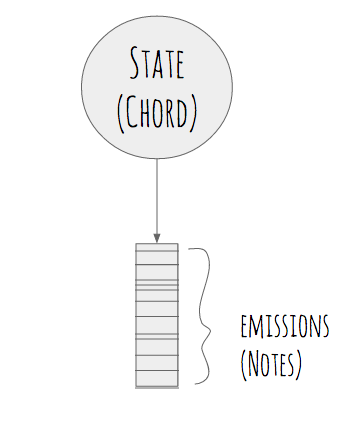
\includegraphics[scale=0.5]{state}
\end{figure}

\begin{figure}
  \caption{Emission + Transition Model}
  \centering
    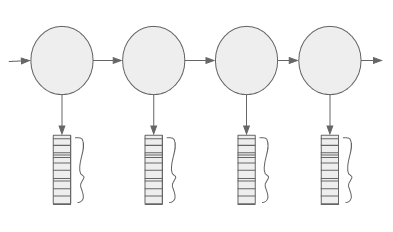
\includegraphics{seq}
\end{figure}

\section{The Data}

The training of any classification system requires supervised data and in the field of music this can be a challenge to source due to copyright issues. Luckily for this project there is a fantastic, openly available database of annotated jazz solo transcriptions made available by The Jazzomat Research Project called the Weimar Jazz Database (WJazzD) \cite[]{wjazz}. The data has been made available since February 20th 2015 and was constructed using an open source audio recording analysis software called Sonic Visualiser \cite[]{sv}. The database contains 299 MIDI transcriptions of jazz solos by famous musicians along with the annotated meta data. Unfortunately, as the data is exclusively from solos improvised over the chord sequences, as opposed to melodies composed with the chord sequences, the notes are less likely to reliably model the chords. This negatively affects the results, as is shown in Chapter 5.

\section{Emission Model}

\subsection{Feature Extraction}

The Emission Model captures the observed data with feature vectors, so the MIDI files must first be processed into these desired features. Also a useful representation must be determined for the annotated chords that are to be used as classification categories.

In western tonal music, songs are generally divided into keys. These tend to be centred on one of twelve possible notes, called the tonic, and are then further modified by being either major, minor or (more rarely) one of seven possible 'modes'. Key information is available for the data used in both training and testing, so to normalise for this a relative representation of pitch was chosen. Specifically each instance of a note or chord is expressed as a Tonal Pitch Class (TPC), a value between 0 and 11, which represents the distance in semitones between the note and the tonic of the piece (i.e. the key). This can be thought of as transposing all the solos to the same key. It should be noted that in doing this both a system of equal temperament is assumed, and absolute pitch data is abstracted away, hence if one note is an octave above another, they are considered the same to be the same TPC. It is possible to account for the variations in mode as in \cite{mysong} but that is not done at this time.

Information regarding pitch is not the only data that is useful in this task, metrical data is also used for the chord tone and concatenation models, see Sections 3.3.2.2 and 3.3.2.3. For this information we adopt the following terminology, introduced by \cite{mel}: the songs are divided into distinct \emph{bars}; each bar in one song contains the same number of \emph{beats}, generally between two and four; each beat can be divided into any number of \emph{divisions}; each individual division is referred to as a \emph{tatum}. As additional features for each note of the melody, the \emph{beat} the note lands on, the number of \emph{divisions} on that beat, the duration of that note in tatums (the \emph{durtatum}) and the current \emph{tatum}, are all used.

On top of this, specific metrical qualities in a note are explicitly modelled. Whether or not the note is \emph{syncopated} (i.e. off the beat) is represented with a binary feature. The \emph{metrical weight} is a measure of how significant a note is metrically and is represented with a ternary feature, zero for a sub-beat event, one for a weak beat event (i.e. on the 'off beat') and two for a strong beat event (i.e. on the 'on beat'). Lastly an alternative metrical system was also tested, introduced by \cite{frieler2007visualizing}, which is based on a circular system with 48 divisions.

With the incorporation of sequential information in mind, models were also used where the feature vectors contained the values of the previous and next notes in the sequence as components.

\subsection{Segment Classification}

The next step is to segment into chordal sections. At the current time, to focus on choosing the best possible emission model, both the training and the test datasets have been segmented into sections of varying sizes at points where it is known there are chord transitions. As mentioned in Chapter 2 there are many existing algorithms for the automatic segmentation of melodies into chordal sections.

Another choice that was made is how fine grained the classification is going to be in terms of the number of chord categories, K. Ideally a model that took into account all possible variations on chords would be preferable, but for the sake of model comparison K is chosen to be 24, capturing major and minor variations. The following encoding is used:

$$
En(note) = 2 * tpc(note) + 1 + type(note)
$$

Where type is 0 if major and 1 if minor. This encoding allows pseudo start and end states of 0 and $N+1$ to be used.

\subsubsection{'Bag of notes' Method}

The initial method attempted for an emission model was a Na\"ive Bayes approach based on \cite{mysong}. This involved creating a smoothed frequency count matrix of the number of times a note was observed given a certain chord. In this model the only data that was made use of was the TPCs, where each segment is represented by a frequency distribution over the notes that occur in that section. This is the most basic model and performed the poorest. This method is analogous to 'bag of words' document classification techniques, hence 'bag of notes'.

\subsubsection{Chord Tone Based Method}

The next method attempted was to divide the problem into two: first determine which notes in the segment are most probable to be chord tones, second to use these chord tones to determine the current chord. This was modelled as two classification tasks, where the first is a binary classification over all notes and the second is a K-class classification over all segments.

The first classification task was implemented using both support vector machines and decision trees and experiments were carried out to determine the best algorithm to use for this task. A function was written which determined, based on the current chord label in the data and the TPC of the current note, whether that note was a chord tone or not. This then allowed for supervised learning with two classes to try and teach a learning algorithm to perform this task without the chord labels.

The second classification task then uses the binary output of the first to select only the notes that have been determined to be part of the chord and then uses these to determine the chord label. The same algorithms were used. The input to these algorithms this time were 12-dimensional indicator vectors, where each component corresponded to a TPC and the value was the number of occurrences of that TPC in the segment, given that it was determined to be part of the chord. For example, if the chord was C Major and the sequences of notes was $[C,D,E,D,C]$ then the input vector to the chord classifier for that bar would be: $[2,0,0,0,1,0,0,0,0,0,0,0]$, where $C$ corresponds to index 0 and $E$ corresponds to index 4.

\subsubsection{HMM - Concatenation Method}

A third method was implemented that involved the the concatenation of smaller HMMs. Essentially each $K$ chord has an HMM model and the song is modelled as a sequence of these HMMs laid end to end. In this case the emission model corresponds to K probabilities of observing the sequence of notes given each chord HMM.

One variable of this model that was tested was the number of states each chord HMM should have. Three separate models were proposed.

For the first model it was decided that the states could model whether the current note was a chord tone or not as this allowed for supervised training of the HMMs, as these labels had already been computed. Hence the HMMs were trained with 2 states.

The second model incorporated metrical information. Each state represented the metrical weight of a note, which had three possible values. Either a note could be on the beat (2), on the off beat (1), or not on a beat (0). Again this allowed for supervised training.

The final method that was implemented used the states to represent the Chord Pitch Class (CPC) of each note. These values were in the range $[0,...,11]$ and corresponded to the value of the pitch relative to the tonic of the current chord. This again allows for supervised learning as CPCs can be calculated during training by subtracting the TPC of the root of the current chord from the TPC of the current note modulo 12.

A future extension to this model could be to allow an EM algorithm to determine the most optimal state representation without using musical theory to inform the choice. This will be attempted in the following year of this project.

The input data for this method only used the TPC values (plus metrical information for model 2) and was a sequence , the size of which varied on the size of the segment.

\section{Transition Model}

The transition model of the system is based on a First order Markov Assumption, where in the generational model, the transition probability into the state that generates the current observations is only dependent on the previous state. In this case the states are the underlying chords. It is clear from the extended structure of a piece of music that this is an extreme generalisation and work has been done into investigating the improvements that can be made from incorporating this kind of musical structure into harmonic analysis \cite[]{struct}. Chapter 6 describes the work that shall be done in the second year of this project to incorporate a more complex transition model.

In this case the transition model is simply a bigram model of chords in the training set and can be trained with a smoothed frequency count of the occurrences of each bigram.

\section{Chord Sequence Generation}

To assign a sequence of chords to each song a method of combining the transition and emission models is required. Specifically the most probable sequence of chords must be determined given the data and the chosen models. To compute this the Viterbi Algorithm was implemented, based on the description in \cite{jur}, see section 4.3.

For testing purposes chord sequences were also produced locally, based only on the emission model. In this case, for each segment, the chord with the highest emission probability was chosen.

\chapter{Implementation}

This chapter will provide a short overview of exactly what was implemented for this project. The programming language used was Python.

\section{Data Manipulation}

The data used for this project was stored in a database and both accessed and pre-processed using software provided by the Jazzomat Research Project \cite[]{mel}. The {\tt melfeature} tool was used, along with others, to created a csv file containing the necessary features for the task, where the rows corresponded to segments, with features for each row including the chord associated with it, the list of TPC values and various metrical statistics that were most helpful with the Chord Tone Model as they provided more features to train on.

\section{Data Loader}

A method of then loading this data into Python was then implemented. The rows of the csv file were loaded into a dictionary which was then iterated over and further processed, see Listing 4.1.

\begin{lstlisting}[frame=single,caption='Data Loader']
def load(self,csv_file_name):

	raw_XX = []
	raw_Y = []

	with open(csv_file_name) as csv_file:
		reader = csv.DictReader(csv_file)
		past_name = None
		X = []
		y = []

		for row in reader:
			
			if past_name != row['filename_sv']:
				if X:
					raw_XX.append(X)
				if y:
					raw_Y.append(y)

				X = []
				y = []

			past_name = row['filename_sv']

			# Get rid of songs with no key
			if not row['key']:
				continue

			# Note: mode not currently used
			key, mode = self._process_key(row)
			self.keys.append(key)
			X_i = self._process_Xi(row)
			y_i = self._process_yi(row)


			# get rid of bars with no chords
			if not y_i:					
            			continue

				X.append(X_i)
				y.append(y_i)

			if X:
				raw_XX.append(X)
			if y:
				raw_Y.append(y)

		self.XX = self._process_XX(raw_XX)
		self.Y = self._process_Y(raw_Y)
\end{lstlisting}

The processing involved the conversion of chord label strings (e.g. 'Cmaj7') into integers in according the labelling system designed in Section 3.3.2. The sequences of notes were similarly processed.

The output of this section was a two dimensional list of chord labels, with the first dimension corresponding to the separate songs, and a four dimensional list of input features, see below for details:

\begin{lstlisting}[frame=single,caption='Input dimensions']
"""
X :	4D Matrix
X[:]			= songs (varying size)
X[:][:] 		= frames (varying size)
X[:][:][:]		= notes
X[:][:][:][:]		= components
"""
\end{lstlisting}

For most algorithms the components for each note only consisted of the TPC value, which as mentioned before was an integer in the range $[0,...,11]$. However for the chord tone model and some variations on the concatenation model, other metrical data was included, making each note's representation a vector, hence the fourth dimension.

\section{Model Implementation}

A Hidden Markov Model class was created, from which all the models were then variations. The Emission and Transition Models were explicitly defined in separate classes, for ease in switching in new models for testing. Each needed to have a method of training itself based on the training data and then for returning log probabilities for use in the viterbi algorithm which was implemented in the manner described in Listing 4.3, based on the description in \cite{jur}.
\begin{lstlisting}[frame=single,caption='Viterbi Algorithm']
def viterbi(self, X):
"""
Viterbi forward pass algorithm
determines most likely state (chord) sequence from observations

X :	3D Matrix

	X[:] 		= frames (varying size)
	X[:][:]		= notes
	X[:][:][:]	= components

Returns state (chord) sequence

Notes:
State 0 	= starting state
State N+1	= finish state
X here is different from X in self.train(X,y), here it is 2D
"""

T = len(X)
N = self.number_of_states

# Create path prob matrix
vit = np.zeros((N+2, T))
# Create backpointers matrix
backpointers = np.empty((N+2, T))

# Note: t here is 0 indexed, 1 indexed in Jurafsky et al (2014)

# Initialisation Step
for s in range(1,N+1):
	vit[s,0] = self.transition_model.logprob(0,s) + self.emission_model.logprob(s,X[0][:])
	backpointers[s,0] = 0

# Main Step
for t in range(1,T):
	for s in range(1,N+1):
		vit[s,t] = self._find_max_vit(s,t,vit,X)
		backpointers[s,t] = self._find_max_back(s,t,vit,X)

# Termination Step
vit[N+1,T-1] = self._find_max_vit(N+1,T-1,vit,X,termination=True)
backpointers[N+1,T-1] = self._find_max_back(N+1,T-1,vit,X,termination=True)

return self._find_sequence(vit,backpointers,N,T)
\end{lstlisting}

\subsection{Emission Model}

There were three main variations on the Emission Model that were implemented.

The first was the Bag of Notes model and creates a frequency matrix based on the notes seen for a given chord in the training data. This is smoothed and normalised to give the conditional probabilities of observing each chord, see Listing 4.4. The base 2 logarithm of this is then returned to the viterbi algorithm.

\begin{lstlisting}[frame=single,caption='Emission Model - Bag of Notes']
def _get_nb_estimates(self, X, y):

	model = dict()

	for state in self.states:
		model[state] = np.zeros(self.dim)
	for i, song in enumerate(X):
		for j, frame in enumerate(song):
			state = y[i][j]
			model[state] += frame

	# Smooth and Normalise
	for state in self.states:
		model[state] += 1
		model[state] = normalize(model[state][:,np.newaxis], axis=0).ravel()

	return model

\end{lstlisting}

The second Emission Model involves two machine learning tasks, the decision on whether a note is in a chord tone or not, and the decision on which chord is most probable given the chord tones observed, as described in Section 3.3.2.2. Section 5.1 details the testing that was done over the various possible algorithms and input features, Listing 4.5 contains only the code for the decision tree model. The Sci-Kit Python Library \cite[]{pedregosa2011scikit}, was used for the implementation of the decision trees. The methods for determining which notes were chord tones in the training data were implemented in {\tt utils.py}.

\begin{lstlisting}[frame=single,caption='Emission Model - Chord Tones']

def _train_chord_tones_dt(self, X, y):

		chord_tones = get_chord_tones(X, y)

		X_np, ct_np = get_concat_ct_X(X, chord_tones)

		self.dt_part1 = DecisionTreeClassifier()
		self.dt_part1.fit(X_np,ct_np)

		X_ct , y_ct = get_ct_features(X, y, chord_tones)

		self.dt_part2 = DecisionTreeClassifier()
		self.dt_part2.fit(X_ct, y_ct)

\end{lstlisting}

The final emission model involved implementing a second type of HMM. These modelled only a segment and one was initialised for each chord. They then output the log probability of that HMM producing the observed sequence of chords. In the higher level HMM the full system is then equivalent to concatenating the smaller HMMs and running the viterbi algorithm over the whole song. In reality, to fit in with the other implementation, the viterbi algorithm is run on each in turn to produce the log probabilities. The implementation of these smaller HMMs can be found in {\tt mini\_hmm.py}. Tests that were done to find the best use of states as a higher level representation at the smaller level are described in Section 5.2.

\subsection{Transition Model}

Only one transition model was implemented for this first half of the project, and is essentially a bigram model over the sequences of chord labels, see Listing 4.6.

\begin{lstlisting}[frame=single,caption='Transition Model']
def _get_normalised_bigram_counts(self,y):

	model = dict()

	for state in self.states:
    	model[state] = np.zeros(self.number_of_states + 2)

		for sequence in y:
			lasts = None
			for state in sequence:
				if lasts is not None:
					model[lasts][state] += 1
				lasts = state

		# Smooth and Normalise
		for state in self.states:
			model[state] += 1
			model[state] = normalize(model[state][:,np.newaxis], axis=0).ravel()

		return model
\end{lstlisting}

\subsection{Template Model}

A variation on the template model proposed by \cite{pardo2002algorithms} was also implemented. This did not require training and simply iterated through song and assigned the chord of the template that best fitted the current segment. The score function that was implemented is given in Listing 4.7.

\begin{lstlisting}[frame=single,caption='Template Model - Score Function']
def score_templates(self, obv):

	score = dict()

	for chord in self.states:
    	if chord % 2 == 0:
			# Minor
			chord_tpc = (chord / 2) - 1
			mode = 0
		else:
			# Major
			chord_tpc = ((chord + 1) / 2) - 1
			mode = 1
		template = (chord_tpc,(chord_tpc + 3 + mode) % 12,(chord_tpc + 7) % 12)
		missing = [1,1,1]
		score[chord] = 0
		for note, dur in obv:
			if note in template:
				score[chord] += (dur + 1)
				idx = template.index(note)
				missing[idx] = 0
			else:
				score[chord] -= (dur + 1)
				score[chord] -= sum(missing)
	
    return score
\end{lstlisting}

\section{Training and Testing}

To train the models 10 Fold cross validation was implemented, using the K-Fold function from SciKit Learn \cite[]{pedregosa2011scikit}. See Listing 4.8 for details. 

\begin{lstlisting}[frame=single,caption='Cross Validation']
def cross_val(self,n=10):
"""
	n : n-crossvalidation
	"""

	XX_train = self.XX_train
	Y_train = self.Y_train

	L = len(self.XX_train)
	kf = KFold(L,n_folds=n)

	models = []
	scores = []

	c = 0

	for c, (train_indexes, val_indexes) in enumerate(kf):

		xx_train = []
		y_train = []
		xx_val = []
		y_val = []
		for i in train_indexes:
			xx_train.append(XX_train[i][:])
			y_train.append(Y_train[i][:])
			
        	for j in val_indexes:
			xx_val.append(XX_train[j][:])
			y_val.append(Y_train[j][:])

		model = HMM()

		model.train(xx_train,y_train)

		count, correct = model.test(xx_val,y_val)

		score = float(correct) / float(count)

		models.append(model)
		scores.append(score)

	max_score = max(scores)

	max_index = 0
    for idx, score in enumerate(scores):
		if score == max_score:
        	max_index = idx
			break

	return models[max_index]
\end{lstlisting}

The testing of the models was done by simple chord by chord comparison of the labelled testing data and the output of the models, reporting back the accuracy.

\chapter{Results}

\section{First Set of Experiments}

The results presented here are from predicting chords without a transition model. The models trained on the two-part chord tone system were a Support Vector Machine (SVM) with an RBF kernel, an SVM with a linear kernel (Lin SVM) and a Decision Tree (DT). A Naive Bayes (NB), 'Bag of Notes' model was also used, predicting chords straight from the data. The experiments were carried out before the full HMM had been built and were done to determine the best machine learning  algorithm to implement into the full architecture.

\subsection{Predicting Chord Tones from Data}

The effects of feature selection were tested over their ability to predict chord tones. The ground truth was automatically computed from the annotated chords. The results are presented in Figure 3.1. 

\begin{figure}
  \caption{\textbf{Accuracy across variations on input features:} \emph{Local} refers to the use of only data from the current note. \emph{Seq} refers to use of additional data from the previous and following note. \emph{B} refers to beat information, \emph{Div} to number of divisions, \emph{D} to 'duratum' and \emph{TPC} to the tonal pitch class.}
  \centering
    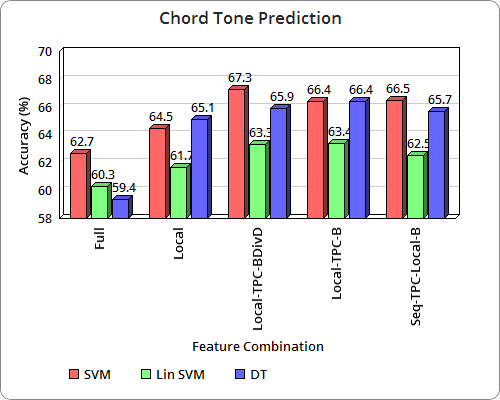
\includegraphics[scale=0.5]{ct1}
\end{figure}

From these results it is clear both that an SVM model achieves the highest accuracy and that Local-TPC-BDivD (see Figure 5.1) was the best combination of features.

These results suggests that the inclusion of sequential data is not beneficial to this form of model. The higher performance of the SVMs is expected as the literature suggests they are a more effective machine learning technique \cite[]{huang2003comparing}. The inclusion of Decision Trees was done as they are much faster to train and test. The fact that lower dimensional models work best isn't surprising as some of these components may not correlate with the task and may just introduce noise. Also machine learning algorithms benefit from a low number of dimensions \cite[]{cortes1995support}.

\subsection{Predicting Chords from Chord Tones}

The input to the learner that takes chord tones to chords is a 12-dim vector for each segment, with each component representing a TPC. Two methods of input were tested, one where each component is a binary indicator of whether the corresponding note is a chord tone in this segment, the other where it is a frequency count of the number of times that note appears as a chord tone in this segment, putting more weight on that note. The results are shown in Figure 5.2.

\begin{figure}
  \caption{\textbf{Accuracy across variations on chord tone representation:} \emph{Bin} refers to the binary representation and \emph{Freq} to the frequency.}
  \centering
    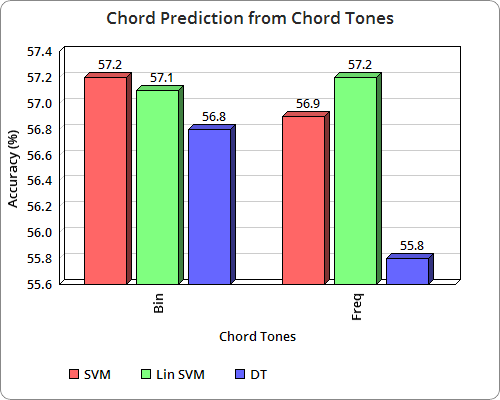
\includegraphics[scale=0.5]{ch}
\end{figure}

The results show that the binary representation is preferable, again with the SVM providing the highest accuracy. The most noticeable effect was on the Decision Tree problem, perhaps because binary decisions produce a better model.

\subsection{Overall Performance of Local Emission Model}

Finally tests were performed combining the systems and compared to a one stage Na\"ive Bayes system and a baseline uniform probability over all classes modelled. Figure 5.3 shows the accuracies and Figure 5.4 contrasts the performance time of each system.

Due to the very slight difference in accuracy between the Decisions Tree and the Support Vector Machines and the very large difference in training and classification time, the Decision Tree model was chosen to integrate into the full HMM.

It is noted that these accuracies are not competitive, but their enhanced performance over a baseline model of uniform chance shows that they represent the emission relationship to some degree. However if a baseline model is instead taken as one which chooses the most frequent chord in the training data, then we see an accuracy of 28.1\%, which is not then beaten by any of the models later tested in this report. This most frequent chord turns out to be the tonic chord. This is further discussed in the conclusion. 

\begin{figure}
  \caption{\textbf{Full Emission Model}}
  \centering
    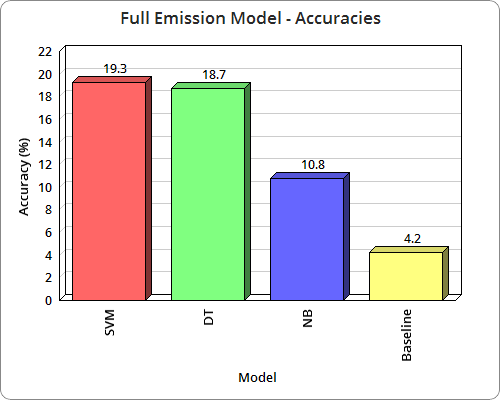
\includegraphics[scale=0.5]{em}
\end{figure}

\begin{figure}
  \caption{\textbf{Training and Testing Times}}
  \centering
    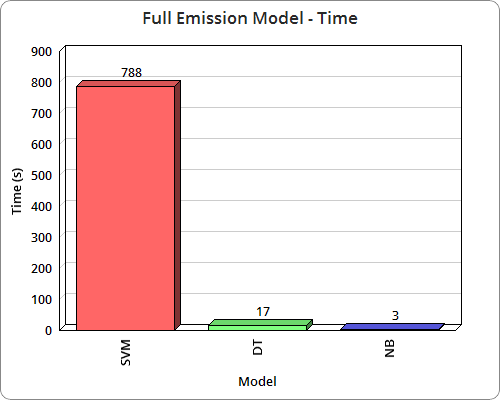
\includegraphics[scale=0.5]{time}
\end{figure}


\section{Second Set of Experiments}

The second set of experiments were carried out on the full HMM, over the three implemented emission models. The transition probabilities were calculated using a bigram count of chord labels, adding the special labels of $start$ and $end$.

A fourth model was also implemented, for comparison, based on the template method proposed in \cite{pardo2002algorithms}. This method compared the segments against triad templates for each chord and generated a score for each, based on how many notes were present both in and not in the template, weighted on duration, and how many notes were in the template and not in the segment. This method did not use any transition models: it selected the highest scoring template for each segment in turn, independent of the others. Implementing this method was very useful in determining the quality of the data, as \cite{pardo2002algorithms} report high accuracies, the best being 88.7\%.

For experiments the dataset was split into a training set and testing set. The training set was two thirds of the total data, consisting of 181 songs, with test set containing the remaining 90. All training was done using 10-fold cross validation on the training set, and all reported accuracies are from classification of the test set.

\subsection{Concat HMM Model}

The three different models of lower level HMM, as described in Section 3.3.2.3, were trained and tested and the results are presented in Table \ref{concat}. The 12 state CPC model was the most effective. This was expected as the transitions between relative pitches hold more information than just the transitions between more significant and less significant notes, which is essentially the aim of the other two models.

\begin{table}
\centering
\caption{Concat HMM Model Results}
\label{concat}
\begin{tabular}{l|l}
Model                           & Accuracy (\%) \\ \hline
2-State HMMs - Chord Tone Model & 18.0          \\
3-State HMMs - Metrical Model   & 19.3          \\
12-State HMMs - CPC Model       & 21.0         
\end{tabular}
\end{table}

\subsection{Model Comparison}

Table 5.2 shows the main results of this report, with the best performances of each model. It is noted that the final accuracies are poor across all models, with the Chord Tone model achieving the best score. This could be caused by many factors but the most probable reason is that the data used for this project, that of solo transcriptions, simply doesn't model the underlying harmonic progression to the same reliability as a written melody would. This is supported by the fact that the template model implemented in \cite{pardo2002algorithms} performs very well, with accuracies higher than 80\%, whereas here it is only the second best model.

Another possibility is the inherent ambiguity of jazz substitutions, this is further discussed in section 5.3.1.

\begin{table}
\centering
\caption{Comparison of best results of each model}
\label{main}
\begin{tabular}{l|l}
Model               & Accuracy (\%) \\ \hline
Bag of Notes HMM    & 3.2           \\
Concat HMM          & 21.0          \\
Chord Tone HMM (DT) & 27.5          \\
Template Model      & 23.7         
\end{tabular}
\end{table}

\section{Further Experiments on Fewer Chords}

As mentioned, the standard set of chords that were used by the models for classification consisted of 24 major/minor variations of the 12 pitch classes. The models were later run on different sets of chords to see how well they could adapt and to further investigate the data.

\subsection{Root Extraction}

First the models were adapted to only detect the root of the chord instead of both the root and the mode (here mode is referring to being either major or minor). This reduced the chord set to 12. The results are presented in Table \ref{12}.

Interestingly we see very little increase in accuracy over the full set, showing that it is not mode classification which the system performs poorly on, but root extraction. This makes sense as with Jazz there are many chords which can be substituted for each other see \cite{granroth2014robust}[p.12] for a comprehensive list. However in this list, note typically that minors are not substituted for majors. This is perhaps less the case in genres other than jazz (i.e. the relative minor substitution). This suggests that it is easier to determine the mode of a chord, rather than its root. This is explored in the next section.

\begin{table}
\centering
\caption{Root Extraction - 12 Chords}
\label{12}
\begin{tabular}{l|l}
Model               & Accuracy (\%) \\ \hline
Bag of Notes HMM    & 22.5           \\
Concat HMM          & 30.7          \\
Chord Tone HMM (DT) & 27.5          \\
Template Model      & 25.4         
\end{tabular}
\end{table}

\subsection{Mode Extraction}

The other test that was conducted on the models was to see how they coped with the very simple task of only classifying whether the current chord was major or minor. This was treated as the same problem with 2 classes. Note that the Chord Tone based Decision Tree model was not able to be fitted to this task.

The results are presented in Table \ref{2}, and are very surprising, given the quality of the data. All models were able to tell 100\% of the time whether the current chord was major or minor. Not a single error was made by either of the three models. This is an exceptionally good result and shows that the solo data reliably models the mode of the current chord, if not the root, and that the models implemented in this project are able to capture this relationship exactly.

\begin{table}
\centering
\caption{Mode Extraction - 2 Classes}
\label{2}
\begin{tabular}{l|l}
Model               & Accuracy (\%) \\ \hline
Bag of Notes HMM    & 100           \\
Concat HMM          & 100          \\
Template Model      & 100         
\end{tabular}
\end{table}

The results support the notion that the system is better at classifying chord types over chord roots, perhaps due to various jazz substitutions. Another possibility is that, as previously discussed, the ability of solos to confer the underlying harmonic structure of a song is not as complete as that of a more definite melody.

In the following year of this project, the possibility of two-stage classification will be explored, where the mode is determined first, followed by the root, as it is clear the former is very accurate.

\chapter{Further Work}

%\section{Remaing Work of Part 1}

%The nest step is to perform the experiments from the previous chapter while incorporating the transition model into the prediction system.

%Currently a method of incorporating local sequential data into the emission model is being investigated. One possibility is to use a Recurrent Neural Network (RNN) for segment classification, where the input is the sequence of notes in that segment.

%Another task is to segment the data automatically. One method that will be attempted is to treat each note as an individual segment and assign a chord to each note, with consecutive assignments of the same chord being treated as one chord in the output sequence. This restricts what can be achieved with the emission model and puts more weight on the transition probabilities. Another method is to uniformly segment the data into sections of equal size, e.g. a bar.

%More machine learning methods for segment classification will also be implemented, including CRFs, Neural Networks and Gaussian Mixture Models.

%Finally further experiments shall be carried out over different variations of the system to test the various parameters and find the most successful model.

\section{Transition Models}

The primary purpose of the second year of this project, as previously mentioned, is to investigate the effects of extended structural analysis with more complex transition models.

One proposed method, and the inspiration for this project, is to adapt a jazz parser presented by \cite{ccg} that currently uses Combinatory Categorical Grammars (CCGs) to analyse jazz chord sequences. As it is a statistical model, it could be adapted to give probabilities of individual chord sequences. This could be combined with an emission model of notes to chords to create a system that could search for the overall most probable harmonic analysis. The idea behind this is that jazz harmonic progressions can rely on long term dependencies and the proposed grammar is very good model of those dependencies. 

Other language models that take into account extended sequential structure and context are those involving Recurrent Neural Networks (RNNs) \cite[]{rnn}. An RNN based approach will also be implemented, in comparison with the grammar model. This will parallel the HMM vs Machine Learning approach taken this year.

A simple improvement to the basic bigram transition model that was presented in this report would be to implement a trigram model with a second order markov dependency. This does not solve the problem of long term dependencies but it is a simple improvement that will show the impact the transition model has on the system.

\section{Data}

The Data provided in the WJazzD is an incredible resource and is very well annotated. However it is perhaps not the best suited to the task of this project, given the nature of jazz solos. For this reason the models of this project will be ran on other datasets, perhaps not necessarily those containing jazz, to confirm this notion.

\section{Expectation Maximisation}

The current transition models rely on HMMs with supervised training. The first improvement that will be made to the system will be to implement the Baum-Welch Expectation Maximisation algorithm \cite[]{baum1970maximization}, to further optimise the models.

\section{Generation}

As the system is a generative model, another possible extension of this project is to implement the generation of jazz melodies for a given chord progression. This would, however, be much more difficult to evaluate as the quality of a jazz melody is a hard to define concept. One possibility is to ask human listeners to score the melodies produced against real jazz melodies.

%In this report the current state of an NLP informed harmonic analysis system has been presented, with details of experiments carried out and further work planned. The final report for this year's work on the project will be presented on Thursday 31st of March, followed by a presentation in the week beginning April 25th.

\chapter{Conclusion}

This report has presented the first year's work of a two year project on the automatic harmonic analysis of jazz melodies. The focus has been on determining the most effective emission model. Three models were proposed, and the one that achieved the highest accuracy was the chord tone based model. However all of the presented models, including the template model of \cite{pardo2002algorithms} achieved very low accuracies. Reasons for this have been proposed and testing on more representative data will show how accurate these reasons are. However it should be noted, as mentioned in Section 5.1.3, that 28.1\% of the labels in the data are the tonic chord, and hence a model that guesses the tonic every time is the most accurate model at this moment. In fact this is near to what happens when the Concat model is run without a transition model, as most segments of the solos look very much like the tonic chord. This will be further investigated in the next year of the project to determine whether this is an unavoidable consequence of the data used.

% use the following and \cite{} as above if you use BibTeX
% otherwise generate bibtem entries

\bibliographystyle{apa}
\bibliography{mybibfile}{}

\end{document}
